\subsection{Overview}
\subsection{Component view}
\begin{figure}[!h]
    \begin{center}
        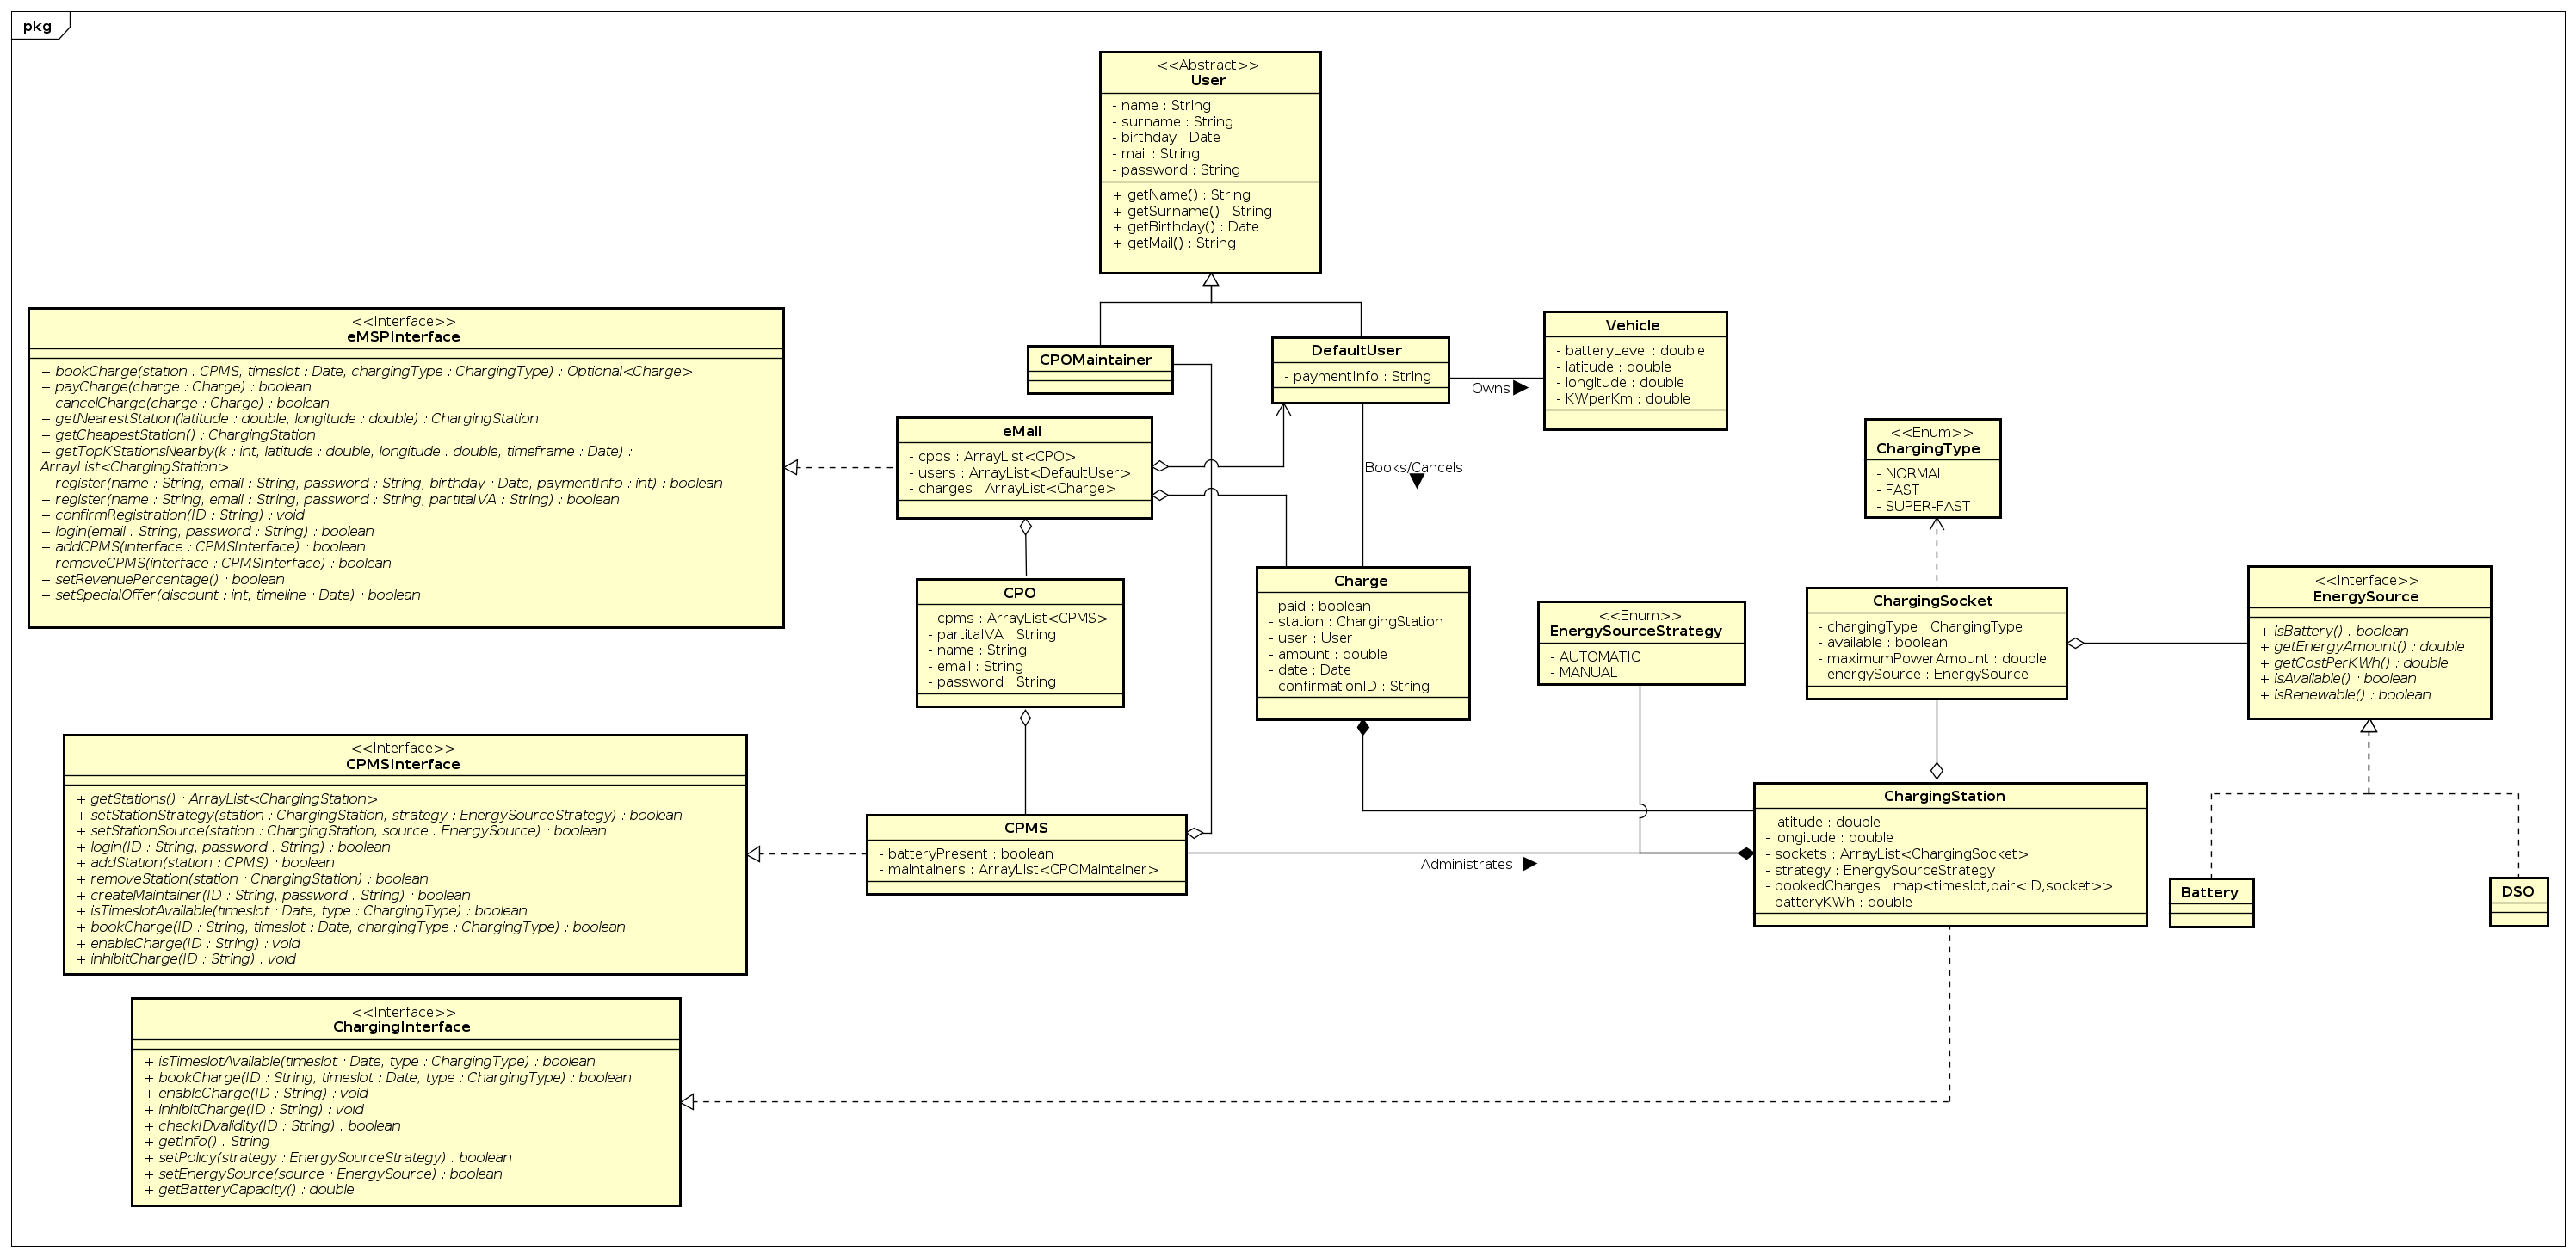
\includegraphics[keepaspectratio, width=16cm]{UML.png}
        \caption{Class diagram}
        \label{fig:UML}
    \end{center}
\end{figure}
In the class diagram illustrated in \autoref{fig:UML} a model (not a functional) view of the system is represented. The \ac{eMall} and \ac{CPMS} interfaces show what the two systems are expected to implement, whereas for the ChargingInterface it is assumed an already existing implementation.
\subsection{Deployment view}
\subsection{Runtime view}
\subsection{Component interfaces}
\subsection{Selected architectural styles and patterns}
\subsection{Other design decisions}
\clearpage